\chapter{Introduction}\label{ch:introduction}

High-energy collider experiments, in particular proton-proton collisions at the Large
Hadron Collider (LHC) at CERN, provide increasingly precise tests of the strong
interaction and of the Standard Model of particle physics. Matching this experimental
precision requires theoretical predictions with correspondingly high accuracy, making
higher-order perturbative calculations in Quantum Chromodynamics (QCD) essential.

QCD is the quantum field theory describing the strong interaction. It is a non-Abelian
gauge theory based on the $SU(3)_c$ colour symmetry, with quarks as fermionic matter
fields and gluons as the corresponding gauge bosons. Quarks occur in six flavours and
transform in the fundamental representation of $SU(3)_c$, while gluons transform in
the adjoint representation and themselves carry colour charge. The quarks and gluons
within the Standard Model particle content are shown in Fig.~\ref{fig:SM}.

\begin{figure}[h!]
    \centering
    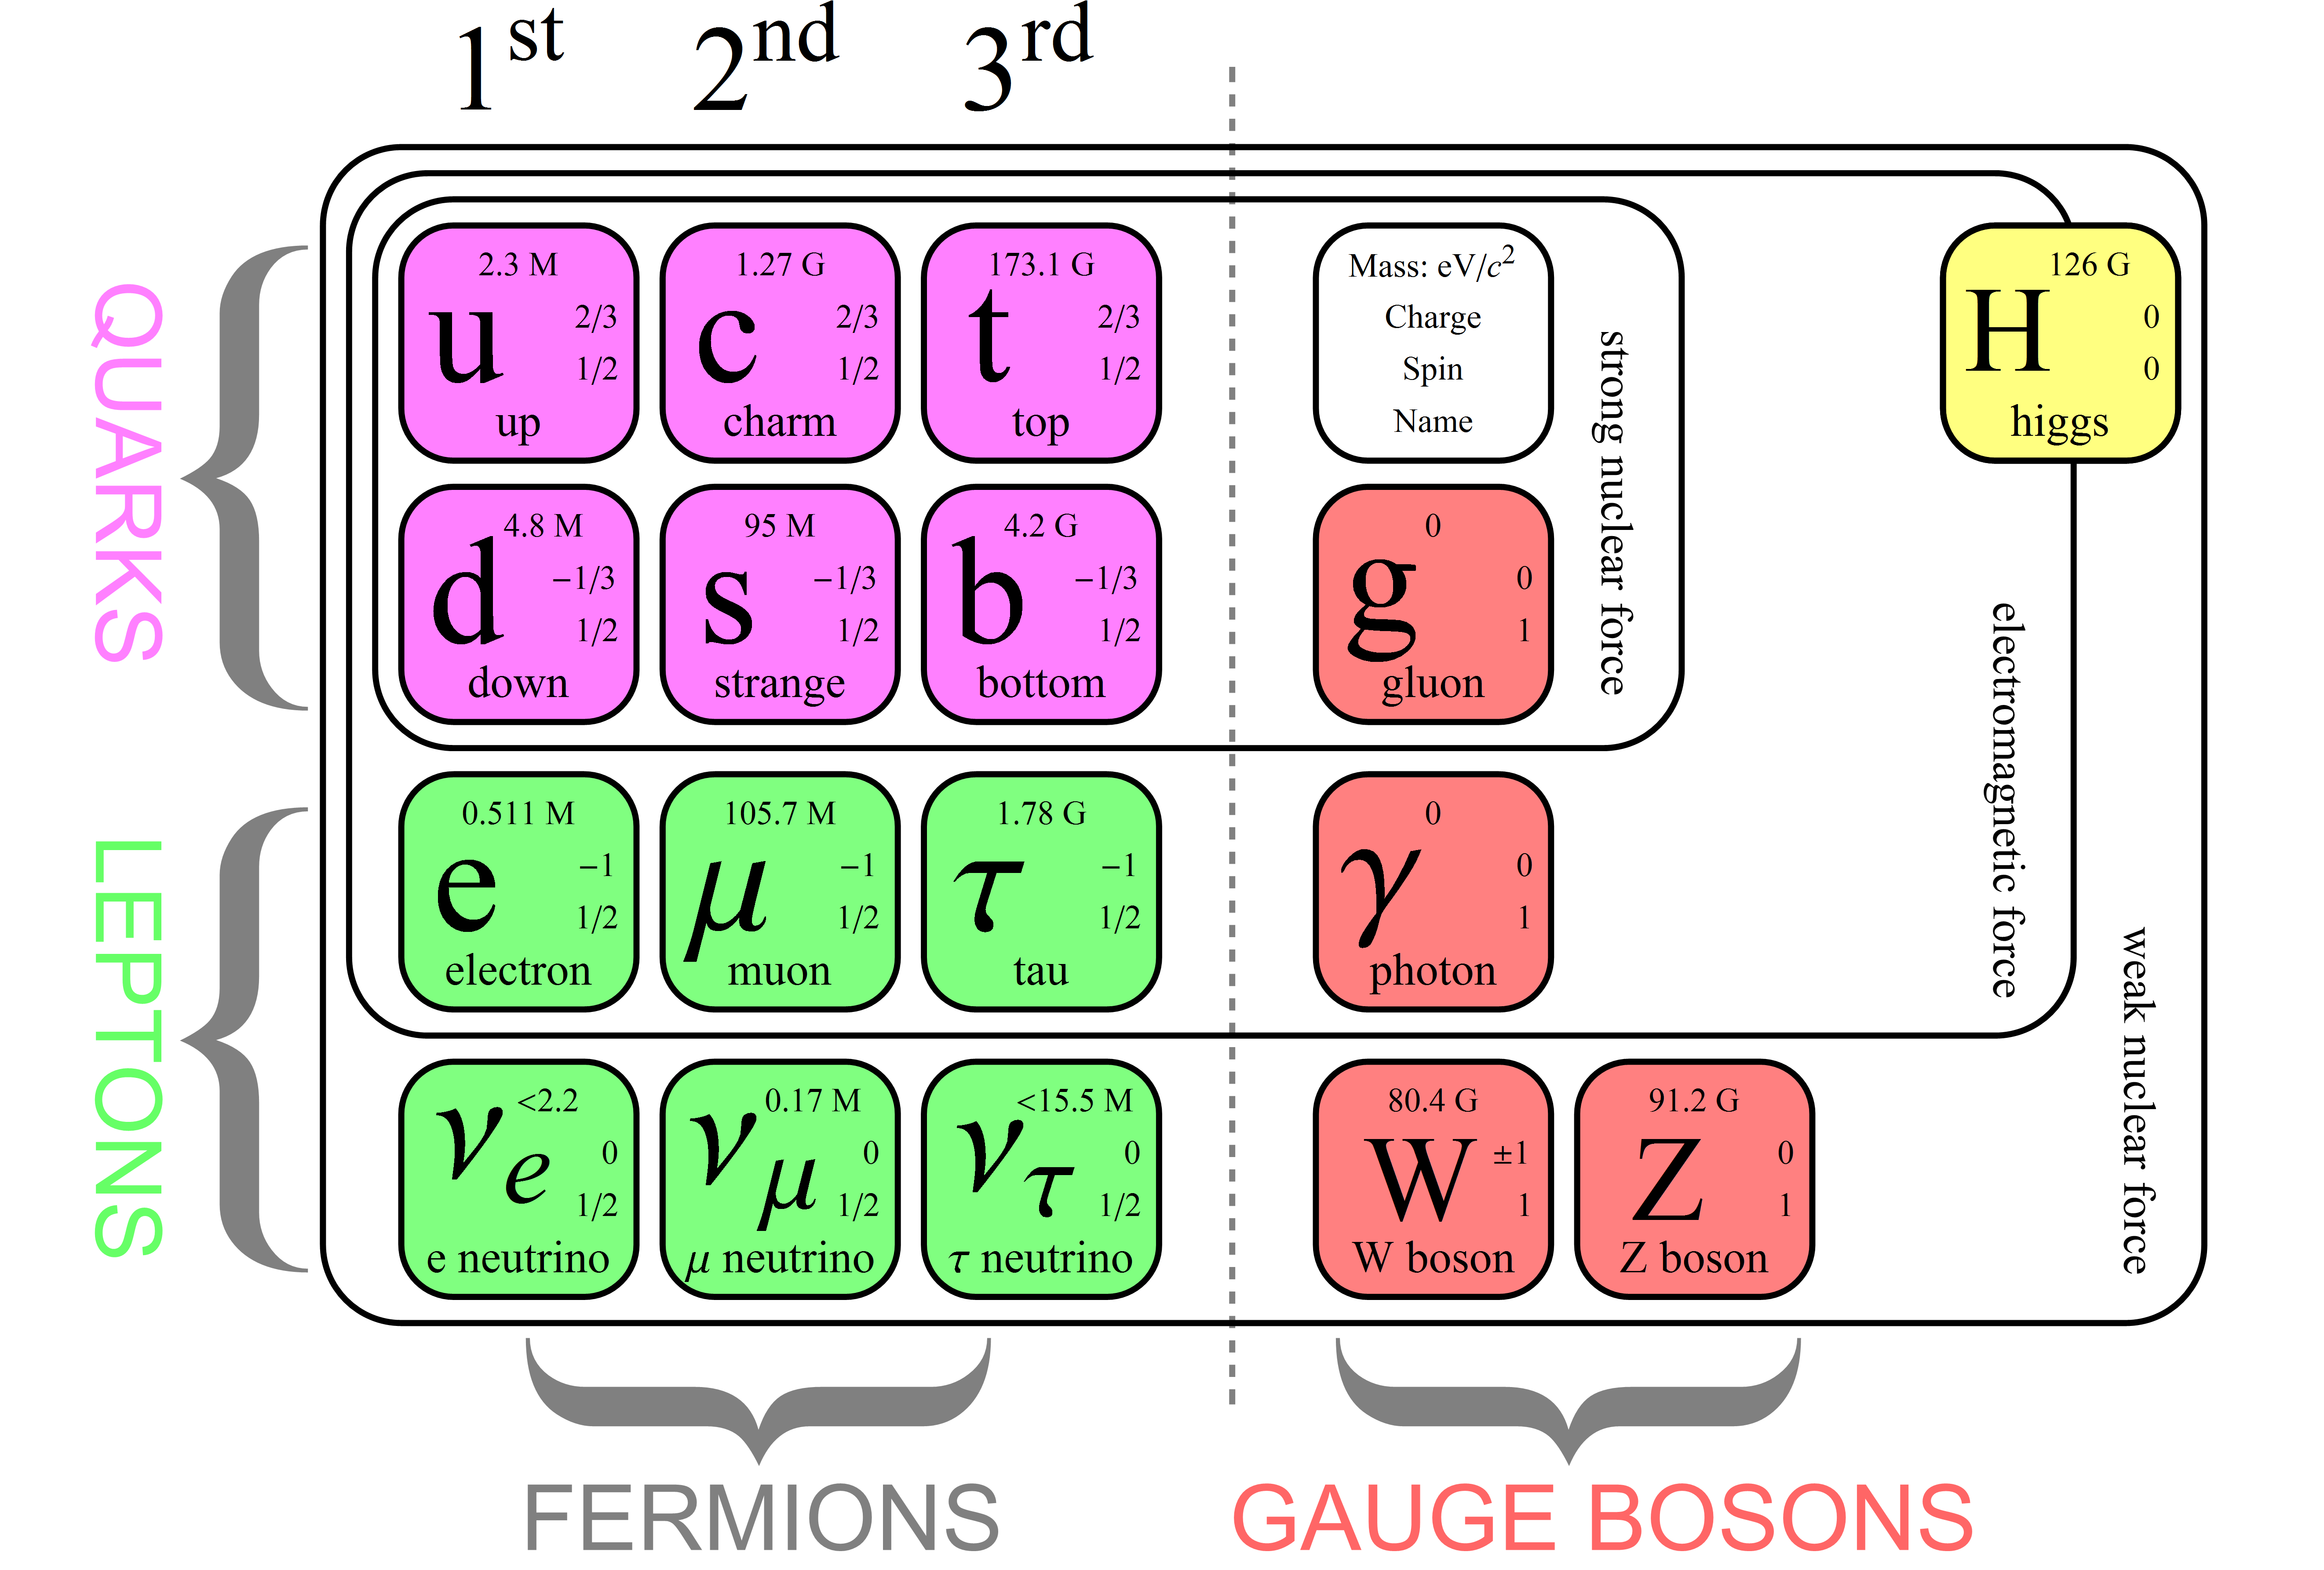
\includegraphics[width=0.9\textwidth]{figures/SM1.png}
    \caption{\centering A diagram representing the Standard Model of Particle Physics. In it, the six quark flavours are 
            visible on the top left in purple, among the fermions, and the gluon is represented close as the topmost 
            gauge bosons, in red. Image by Matic Lubej~\cite{lubejStandardModel}.}
    \label{fig:SM}
\end{figure}

At sufficiently large momentum-transfer scales, the strong coupling $\alpha_s$ becomes
small as a consequence of asymptotic freedom. This allows QCD observables involving a
hard scale $Q$ to be calculated perturbatively as an expansion in powers of
$\alpha_s(Q)$. Successive perturbative orders---leading order (LO), next-to-leading
order (NLO), next-to-next-to-leading order (NNLO), and beyond---generally improve the
accuracy of theoretical predictions and reduce their residual dependence on unphysical
renormalisation and factorisation scales. This improvement, however, comes with a
rapid increase in the complexity of the required calculations.
Obtaining higher-order
perturbative predictions is not simply a matter of calculating
additional Feynman diagrams. Real-emission and virtual-loop contributions develop
infrared singularities in kinematic configurations involving soft (low energy)
or collinear partons. These individual contributions are divergent, and their
infrared singularities must be extracted and cancelled before numerical integration
can be performed. For infrared-safe observables, such as the hadronic \textit{R}-ratio defined in
Chapter~\ref{ch:validation}, the singularities cancel between the real and virtual
contributions, leaving a finite physical result.

The antenna subtraction formalism provides a framework for extracting and cancelling
these infrared singularities, rendering the individual contributions suitable for
numerical integration. The formalism describes unresolved radiation between pairs of
colour-connected hard partons through universal antenna functions. These functions
reproduce the relevant infrared limits locally and, after analytic integration over the
unresolved phase space in dimensional regularisation, $d=4-2\epsilon$,
yield Laurent series whose $\epsilon$-pole structure cancels that of the
virtual contributions.
Their systematic construction and integration are therefore central to higher-order
QCD calculations within the antenna subtraction framework.

This thesis develops and validates \textit{AntCalc}, a symbolic framework for the 
automated construction and integration of QCD antenna functions. The work focuses 
on massless final-final quark-antiquark antennae through next-to-next-to-leading
order (NNLO), combining symbolic amplitude generation with reduction methods for 
phase-space integrals. The resulting implementation is tested globally through the calculation of the
massless hadronic \textit{R}-ratio, a well-known inclusive observable in $e^+e^-$
annihilation that provides a benchmark for the complete implementation, up to NNLO. Locally,
individual antenna functions are tested, where appropriate, by verifying that they
reproduce the expected eikonal factors and Altarelli-Parisi (AP) splitting functions
in the relevant unresolved limits. 

The remainder of the thesis is organised as follows. Chapter~\ref{ch:physicsbackground}
introduces the theoretical foundations required throughout this work, including
perturbative QCD, infrared singularities, dimensional regularisation, and the antenna
subtraction formalism. It defines the massless antenna functions and discusses their
colour structure, phase-space factorisation, and role in fixed-order calculations. The
chapter also introduces the normalisation conventions used throughout. 
Chapter~\ref{ch:packageframework} describes \textit{AntCalc}'s framework, including its
architecture, antenna construction and integration workflows, reduction procedures, and
the conventions and validation tools used to obtain the results.
Chapter~\ref{ch:workedexample} presents the antenna functions obtained using
\textit{AntCalc}, organised by final-state multiplicity, with the master integrals
required for each antenna set presented after the corresponding antennae.
The $A_3^0$ antenna is discussed in detail, from its unintegrated construction to its
integrated form and the validation of its soft and collinear limits. Selected NLO and
NNLO antenna results are then presented more concisely. The chapter concludes with an
exploratory extension of the $A_3^0$ antenna to the massive case.
Chapter~\ref{ch:validation} provides a global validation of the framework through the
calculation of the massless hadronic \textit{R}-ratio through NNLO. The relevant antenna
contributions are combined, demonstrating the cancellation of infrared poles and
agreement with the known finite result.
Finally, Chapter~\ref{ch:conclusion} presents the conclusions of the thesis and discusses
future directions for \textit{AntCalc}, including more efficient symbolic and reduction
backends, completion of the massive antenna sector, further antenna families and kinematic
configurations, and extensions to higher perturbative orders, particularly N$^3$LO.